%! TEX root = main.tex
\section{Results: validations and showcases}

\subsection{Regression test and validation: Malpasset dam-break problem}

We developed \geoclawlandspill{} by modifying and extending \geoclaw{}.
Whenever a simulation does not require any new functionalities, \geoclawlandspill{} should behave the same as \geoclaw{} does.
In this subsection we present a regression test to verify that our modifications do not introduce new bugs into the core SWE solver.
This test also serves as a validation test to the core SWE solver.

The Malpasset dam-break happened in southern France in 1959.
This incident has become a standard validation case for SWE solvers because of the detailed field survey data.
Figure \ref{fig:malpasset-topo-gauges} shows the digitalized elevation model (i.e., topography) and locations where we have real-world data.
We obtained the topography data from the validation package of Telemac-2D (\url{www.opentelemac.org}).
Points P1 to P17 on figure \ref{fig:malpasset-topo-gauges} indicate where the field survey data are available.
Points S6 to S14 indicate the gauge measurements from a lab experiment on a scaled-model.
For the description and the coordinates of these data points, please refer to Biscarini et al. (\cite{biscarini_simulation_2016}).

\begin{figure}
    \centering
    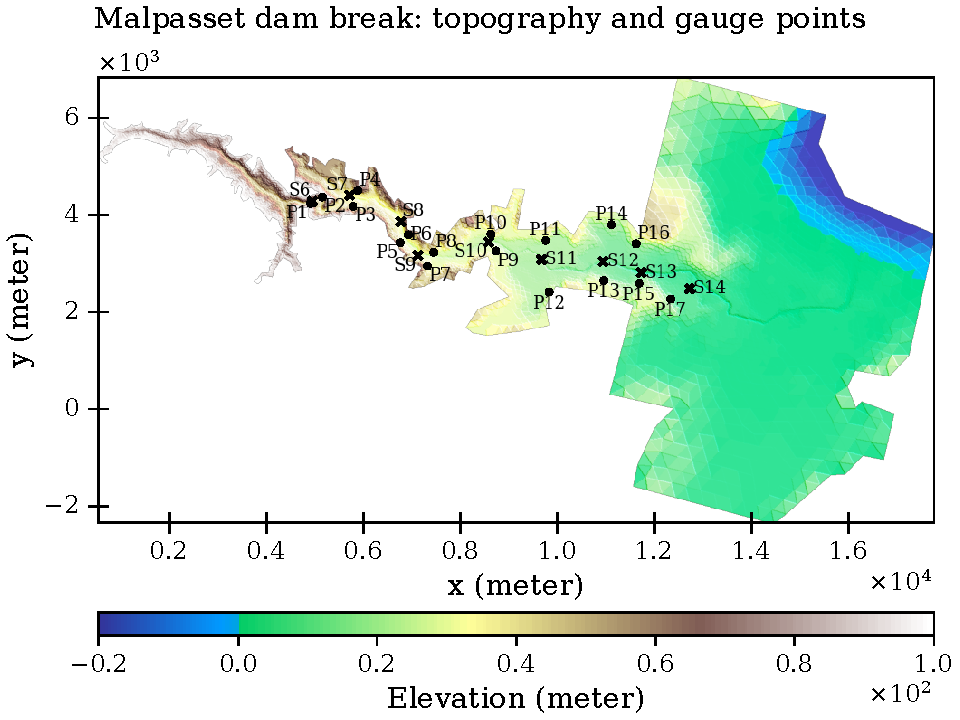
\includegraphics[width=0.9\linewidth]{malpasset-topo-gauges}
    \caption{Topography model and locations of gauges and field survey points}\label{fig:malpasset-topo-gauges}
\end{figure}

Figure \ref{fig:malpasset-gauge-field-survey} shows the maximum water surface levels at field survey locations.
Figure \ref{fig:malpasset-gauge-model} and figure \ref{fig:malpasset-arrival-time} show the maximum water surface levels and water arrival time at the scaled-model's gauges in the experiment.
We compared the simulation results from upstream \geoclaw{} and our \geoclawlandspill{} against the survey/experimental data.
We also compared against the result from GeoClaw in 2011 (\cite{George2011}).
The result from \geoclawlandspill{} agrees with that from upstream \geoclaw{}, which verifies that no bug was introduced.
The result from 2011 \geoclaw{}, however, has a slight discrepancy from our simulation results.
Compared to the field survey and the lab experiment, the simulation results have worse agreement with P1, P13, S6, and S9 on water surface level.
At gauge S14, the simulated arrival time deviates from the lab experiment.

\begin{figure}
    \centering
    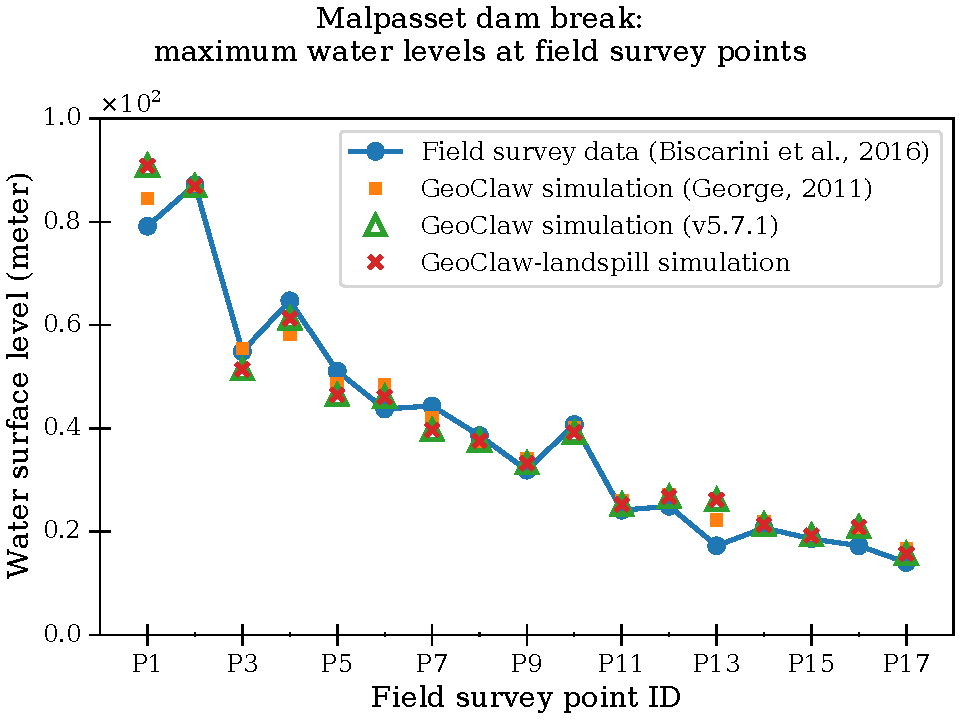
\includegraphics[width=0.9\linewidth]{malpasset-gauge-field-survey}
    \caption{Maximum water surface level at field survey locations}\label{fig:malpasset-gauge-field-survey}
\end{figure}

\begin{figure}
    \centering
    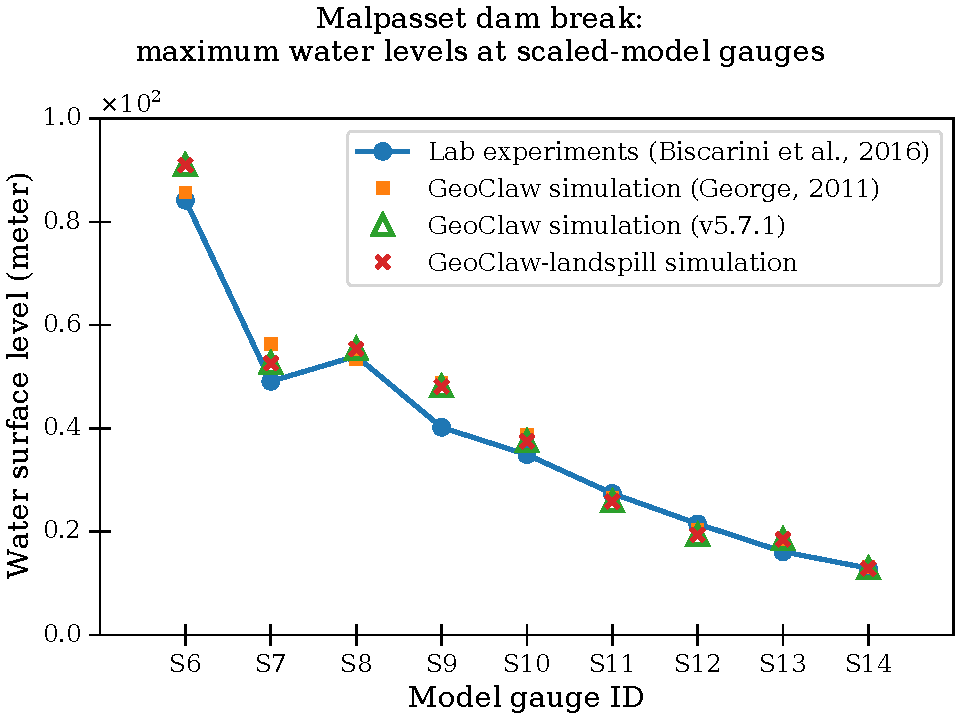
\includegraphics[width=0.9\linewidth]{malpasset-gauge-model}
    \caption{Maximum water surface level at scaled-model gauges}\label{fig:malpasset-gauge-model}
\end{figure}

\begin{figure}
    \centering
    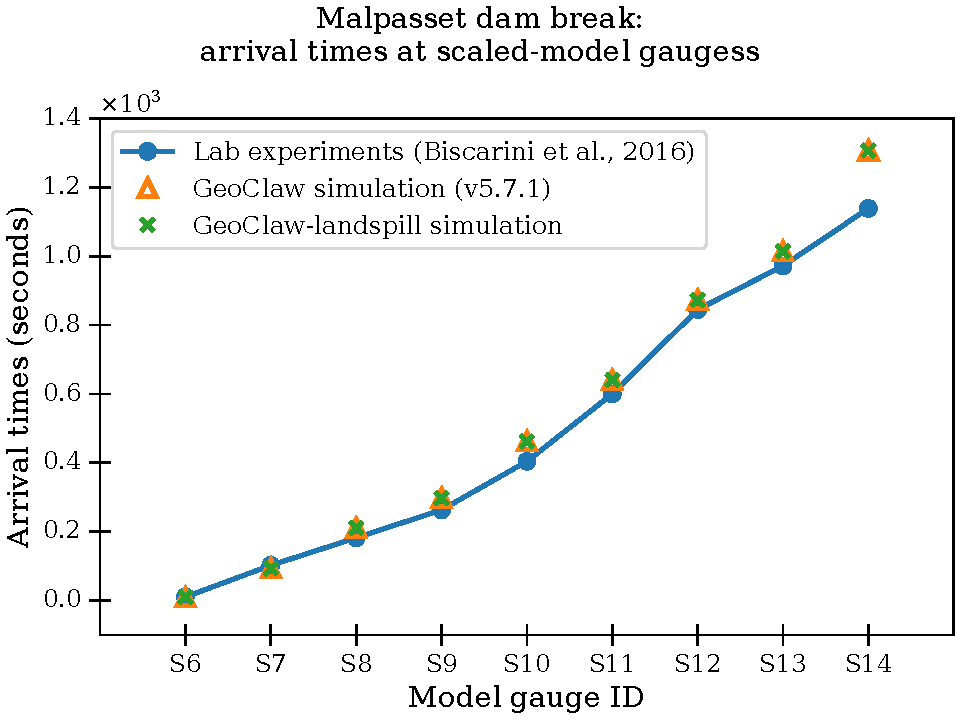
\includegraphics[width=0.9\linewidth]{malpasset-arrival-time}
    \caption{Water arrival times at scaled-model gauges}\label{fig:malpasset-arrival-time}
\end{figure}

\subsection{Validation: silicone oil on an inclined glass plate}

\begin{table}
    \caption{Viscosity ($\mu$), density ($\rho$) and evaporation coefficients ($C_1$ \& $C_2$) of the fluids}\label{table:fluid-properties}
    \begin{threeparttable}
        \begin{tabular*}{\tblwidth}{@{} LRRR@{} }
            \toprule
            & $\mu$ ($cP$) & $\rho$ ($kg/m^3$) & ($C_1$, $C_2$). \\
            \midrule
            Silicone    & 1096.1 & 970 & N/A \\
            Maya crude  & 322 & 926.6 & ($1.38$, $0.045$) \\
            Gasoline    & 0.6512 & 800 & ($13.2$, $0.21$) \\
            \bottomrule
        \end{tabular*}
        \begin{tablenotes}\footnotesize
            \item[*] Maya crude oil's and gasoline's properties are defined at 15\degree{} C.
                Silicone's properties are defined at an unknown temperature.
            \item[$\dagger$] References:~\cite{fingas_appendix_2015}.
        \end{tablenotes}
    \end{threeparttable}
\end{table}



\begin{figure*}
    \centering
    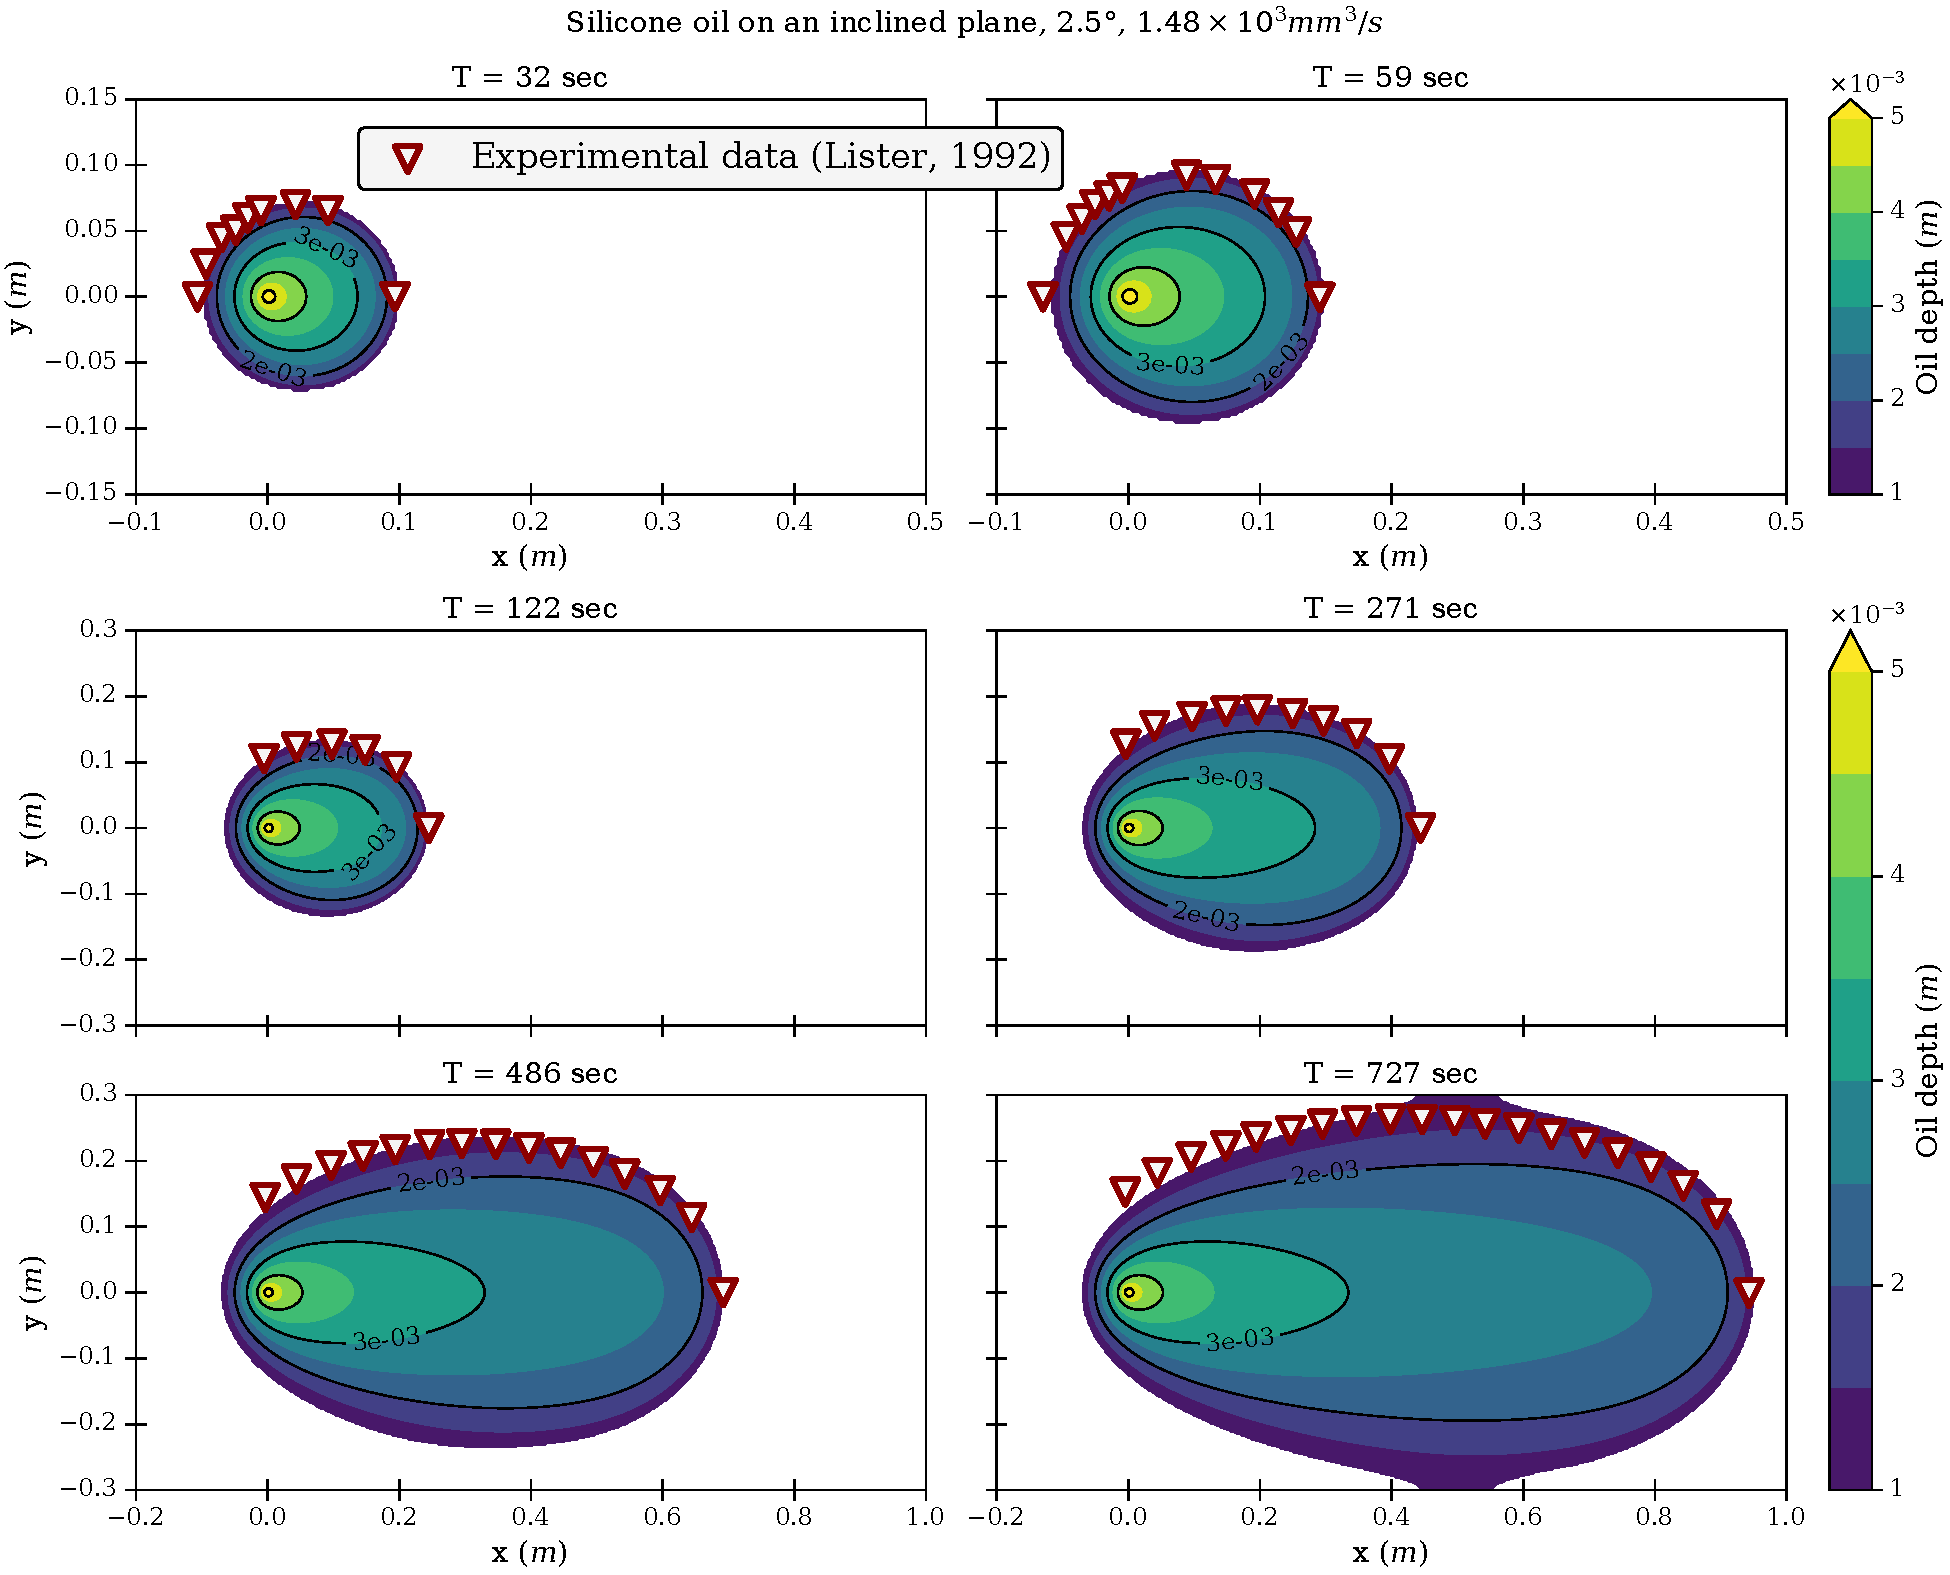
\includegraphics[width=\textwidth]{landspill-silicone-inclined-plane}
    \caption{%
        A validation case of silicone oil on an inclined plane: $angle=2.5\ \mathrm{\degree}$, $flow\ rate=1.48\times 10^{-6}\ \mathrm{m^3/s}$, $outflow\ location=(0, 0)$, $surface\ roughness=0\ \mathrm{m}$, and $ambient\ temperature=25\ \mathrm{\degree C}$. %
        The silicone oil have the following properties: $\mu=1096.1\ \mathrm{cP}$ at $25\ \mathrm{\degree C}$ and $\rho=970\ \mathrm{kg/m^3}$ at $15\ \mathrm{\degree C}$. %
        Note the difference in the coordinate scales in sub-figures. %
        Lister did not mention the flow thickness at the flow front. %
        In this simulation results, we use $1\times 10^{-3}\ \mathrm{m}$ to determine the flow front.%
    }\label{fig:landspill-silicone-inclined}
\end{figure*}

\subsection{Showcase: Maya crude oil and gasoline above flat terrain}

\begin{figure}
    \centering
    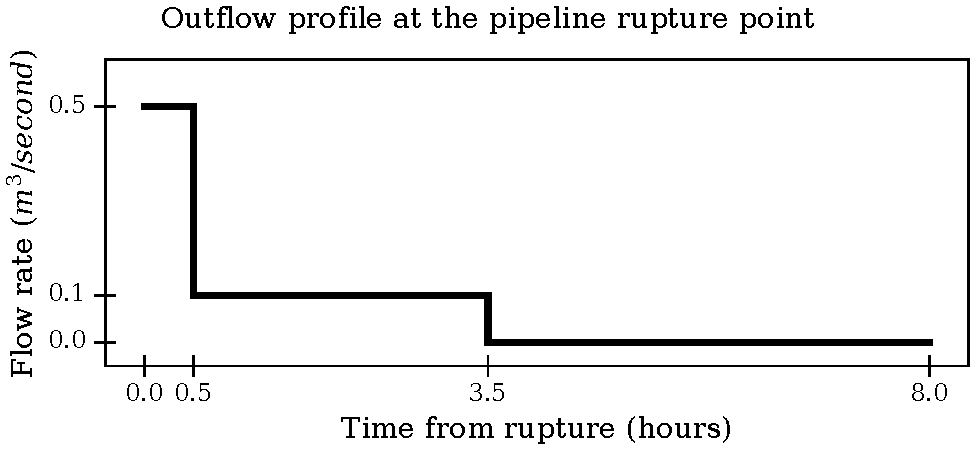
\includegraphics[width=0.9\linewidth]{landspill-outflow-profile}
    \caption{Outflow profile at the pipeline rupture point}\label{fig:outflow-profile}
\end{figure}

\begin{figure}
    \centering
    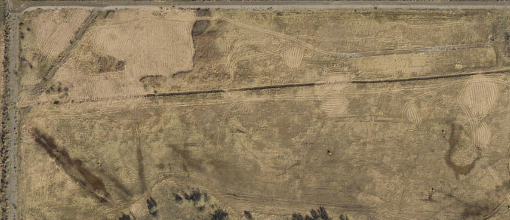
\includegraphics[width=0.9\linewidth]{flat}
    \caption{%
        A flat terrain near Salt Lake City, Utah. %
        Extent (left, bottom, right, top) in EPSG3857: $(-12459905, 4985865, -12459395, 4986085)$.
    }\label{fig:flat-terrain-satellite}
\end{figure}

\begin{figure*}
    \includegraphics[width=\textwidth]{landspill-maya-gasoline-flat-terrain}
    \caption{%
        Maya crude oil and gasoline above flat terrain near Salt Lake City, Utah. %
        The pipeline rupture point, i.e., the outflow location, is located close to the center of each plot. %
        Maya crude oil has higher viscosity than gasoline. %
        The flow, however, is not affected by the viscosity at the beginning stage, where the inertia dominates the flow due to the high outflow rate from the rupture point. %
        In later stages, the outflow rates becomes much smaller. %
        The evaporation rates start to play a much important role than the viscosity does. %
        Evaporation affects the volume of fluid above ground and then further affects the bottom friction, where the viscosity comes into play in SWEs.%
    }\label{fig:landspill-maya-gasoline-flat}
\end{figure*}

\subsection{Showcase: Maya crude oil in drainage terrain}

\begin{figure}
    \centering
    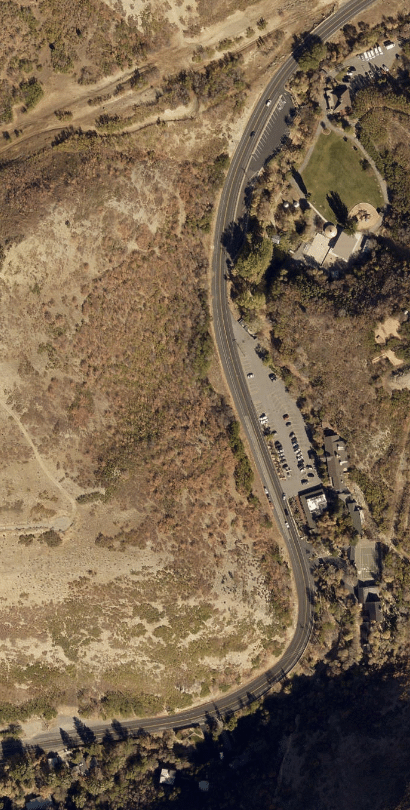
\includegraphics[width=0.7\linewidth]{hill}
    \caption{%
        A hill area near Salt Lake City, Utah. %
        Extent (left, bottom, right, top) in EPSG3857: $(-12443674, 4976959, -12443264, 4977769)$.
    }\label{fig:hill-terrain-satellite}
\end{figure}

\begin{figure*}
    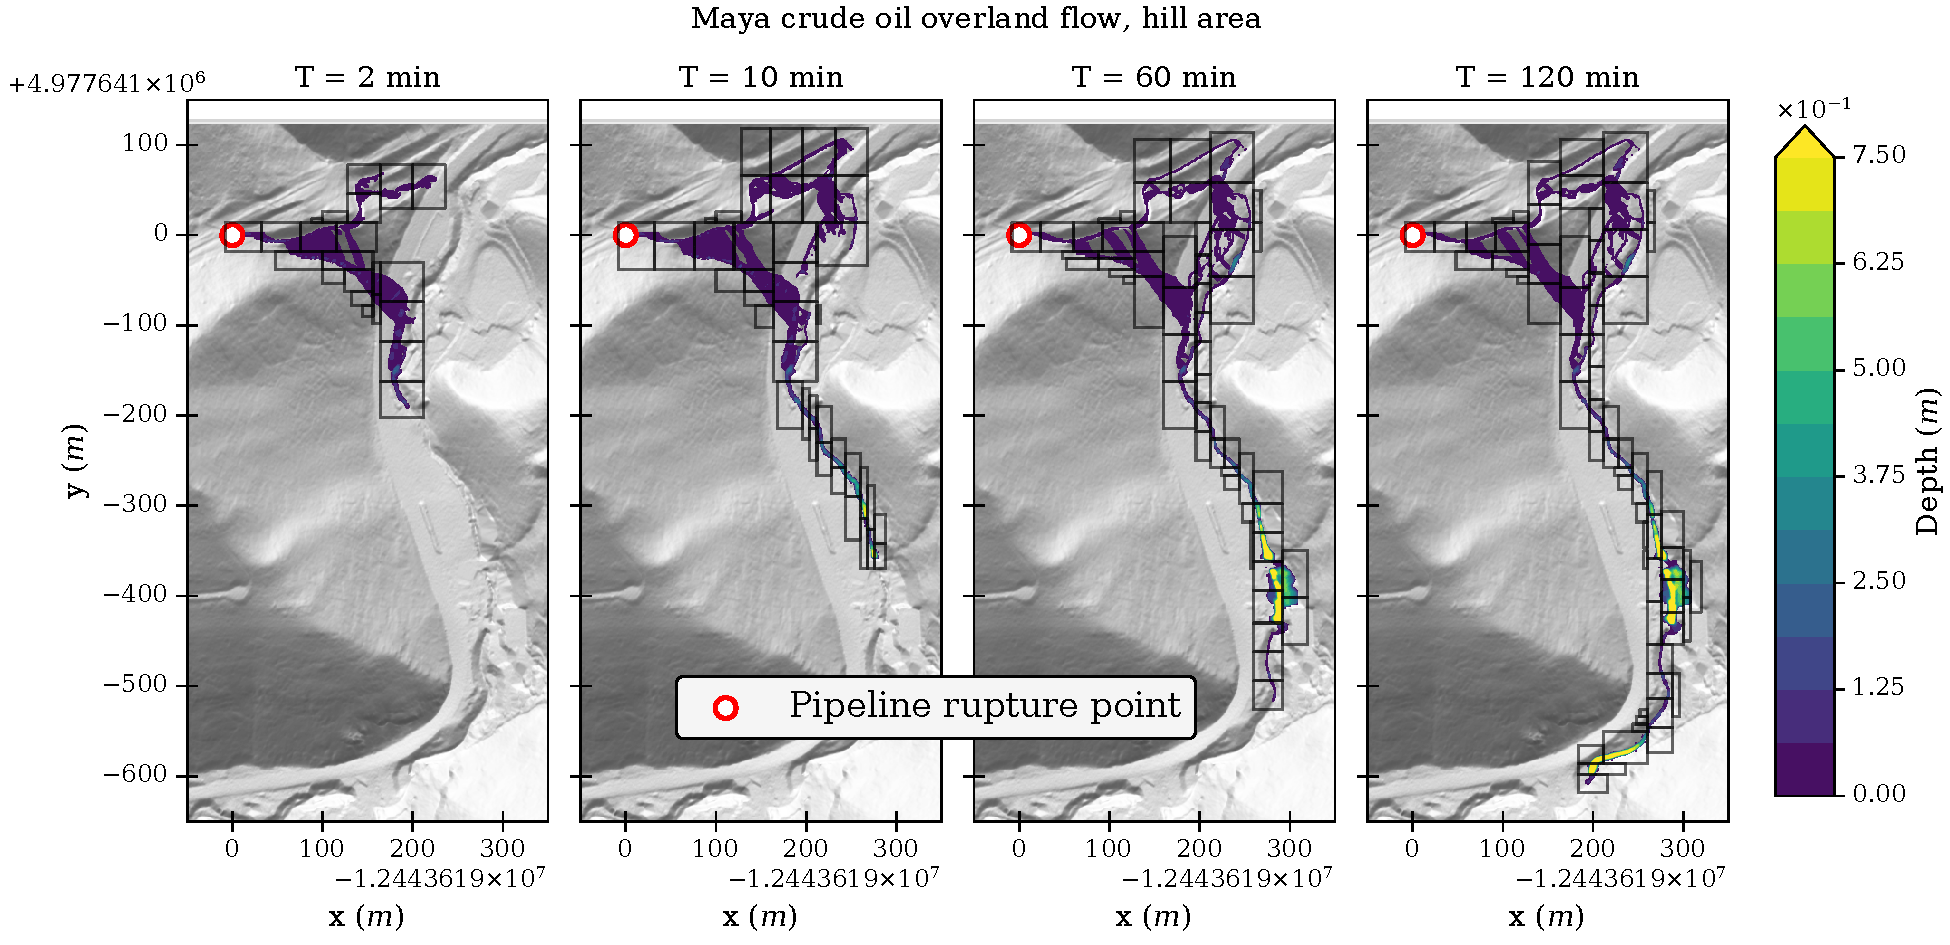
\includegraphics[width=\textwidth]{landspill-maya-hill}
    \caption{%
        Maya crude oil in a hill area near Salt Lake City, Utah. %
        The boxes shown in the figures indicate where the AMR high-resolution grid patches are. %
        In hill areas, flow patterns usually consist of thin but long streams. %
        Resolving the streams with Cartesian grids requires high-resolution grids everywhere in computational domains. %
        And simulations waste much computing power and time because the majority of the grid cells do not have fluid. %
        The use of AMR helps the calculation performance of this type of flows. %
        AMR applies high-resolution grid patches to regions with fluid, while dry regions still use low-resolution grids.%
    }\label{fig:landspill-maya-hill}
\end{figure*}

\subsection{showcase: Maya crude oil in contact with inland water bodies}

\begin{figure}
    \centering
    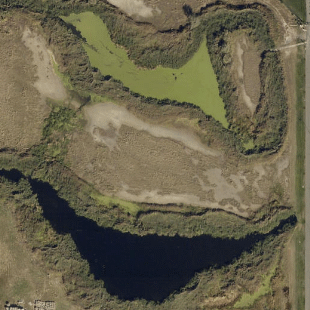
\includegraphics[width=0.7\linewidth]{hydro}
    \caption{%
        An area near Salt Lake City, Utah that has an in-land water body. %
        Extent (left, bottom, right, top) in EPSG3857: $(-12460364, 4984982, -12460054, 4985292)$.
    }\label{fig:hydro-terrain-satellite}
\end{figure}

\begin{figure*}
    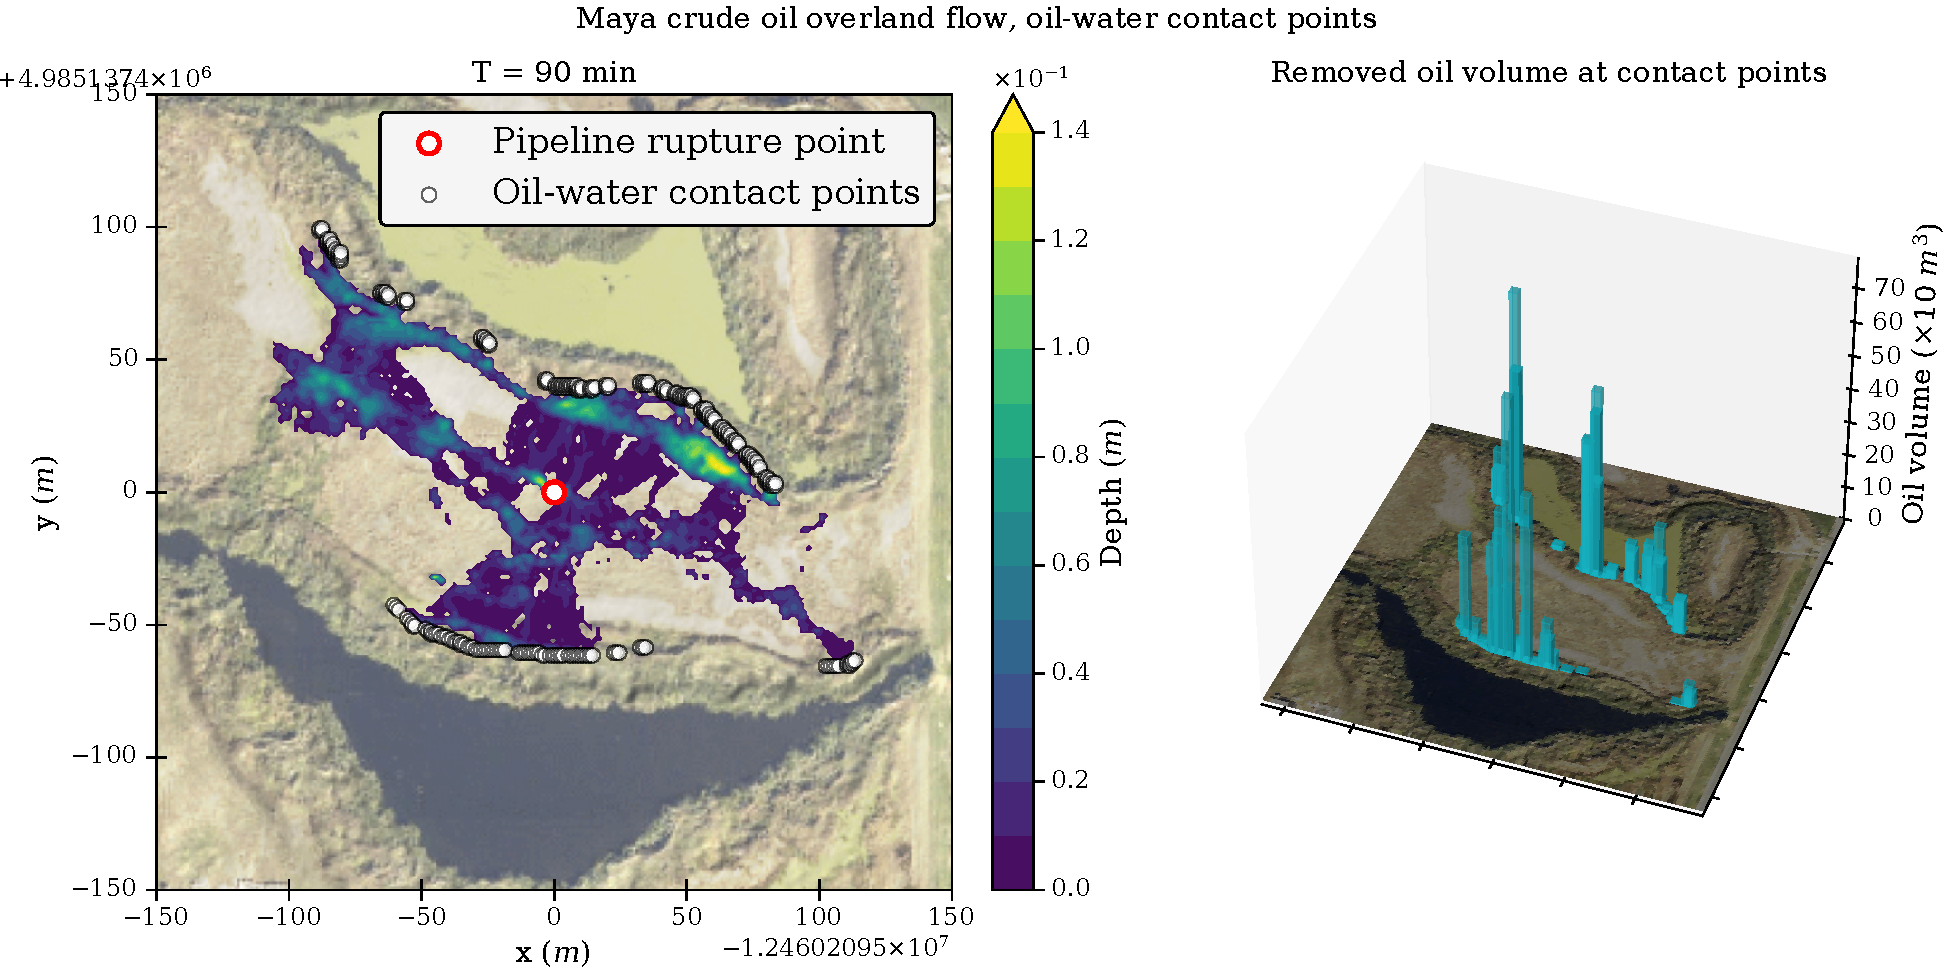
\includegraphics[width=\textwidth]{landspill-maya-hydro}
    \caption{%
        Maya crude oil in contact with water bodies. %
        \geoclawlandspill{} only simulates oil flow above land and does not have hydrographic transport analysis. %
        However, whenever oil flow encounters in-land water bodies, \geoclawlandspill{} records the location of the oil-water contact and the time history of the oil volume flowing into water at each contact location.  %
        These data can be used as the boundary conditions in other third-party hydrographic transport simulation software.%
    }\label{fig:landspill-maya-hydro}
\end{figure*}
% vim:ft=tex:
